\subsection{Упражнение 1}

Скачайте с сайта http://freesound.org , включающий музыку, речь или иные звуки, имеющие четко выраженную высоту. Выделите примерно полусекундный сегмент, в котором высота постоянна. Вычислите и распечатайте спектр выбранного сегмента. Как связаны тембр звука и гармоническая структура, видимая в спектре?


\noindent Используйте high\_pass, low\_pass, и band\_stop для фильтрациитех или иных гармоник. Затем преобразуйте спектры обратно в сигнал и прослушайте его. Как звук соотносится с изменениями, сделанными в спектре?
    

Загружаем звуки игры на пианино, взятые на сайте freesound.org и загруженные на мой репозиторий, после читаем звуки в специальный Wave класс и вырезаем фрагмент.

\begin{lstlisting}[language=Python]
if not os.path.exists('164718__bradovic__piano.wav'):
    !wget https://github.com/wooftown/spbstu-telecom/raw/main/Content/164718__bradovic__piano.wav
wave = read_wave('164718__bradovic__piano.wav')
wave.make_audio()
wave = wave.segment(18.3,0.5)
wave.make_audio()
read_wave('164718__bradovic__piano.wav').plot()
wave.plot()
\end{lstlisting}
    
\begin{figure}[H]
	\begin{center}
		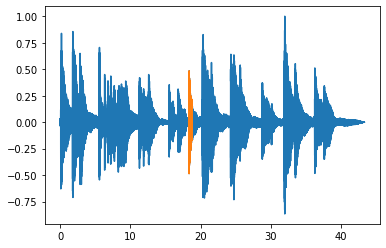
\includegraphics[scale=1]{fig/lab01/lab01_9_0.png}
		\caption{График фрагмента звука}
	\end{center}
\end{figure}

При помощи метода make\_spectrum вычислим спектр звука, и для удобства построим график.
\begin{lstlisting}[language=Python]
spectrum = wave.make_spectrum()
spectrum.plot(high=5000)
\end{lstlisting}

\begin{figure}[H]
	\begin{center}
		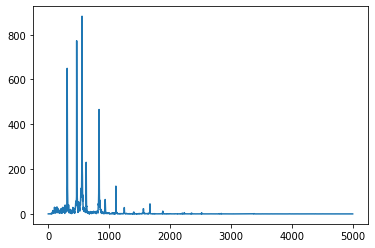
\includegraphics[scale=1]{fig/lab01/lab01_11_0.png}
		\caption{Спектр звука}
	\end{center}
\end{figure}

Можно задать максимальную частоту для графика:

\begin{figure}[H]
	\begin{center}
		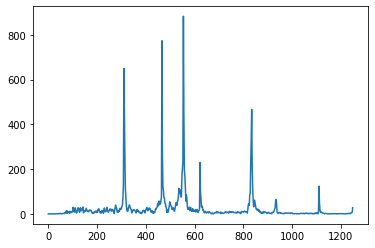
\includegraphics[scale=1]{fig/lab01/lab01_13_0.png}
		\caption{Спектр звука, частота меньше 1250 ГЦ}
	\end{center}
\end{figure}

Для точного понимания какие ноты сыграны выведем список пиков частот в спектре:

\begin{lstlisting}[language=Python]
spectrum.peaks()[:10]
\end{lstlisting}

\begin{lstlisting}
[(882.3500533686324, 554.0),
 (772.8812508117549, 466.0),
 (649.662314039115, 310.0),
 (466.0353893832775, 834.0),
 (455.88324114785496, 312.0),
 (435.6400663619303, 556.0),
 (328.0318016013845, 832.0),
 (260.99365239113706, 314.0),
 (251.02745102094198, 468.0),
 (234.35739758178494, 552.0)]
\end{lstlisting}


Находим соответствие музыкальных нот и частот из пиков:
\begin{itemize}
\item 554.36 Гц - До-диез второй октавы
\item 466.16 Гц - Ля-диез первой октавы
\item 311.13 Гц - Ре-диез первой октавы
\item 830.60 Гц - Соль-диез второй октавы
\end{itemize}
У До-диез второй октавы самая большая амплитуда, поэтому 554.36 Гц - доминирующая частота. Общая воспринимаемая высота звука зависит от основной частоты, тут о
на 311.13 Гц.

Добавим фильтр нижних частот. Все компоненты выше 540 ГЦ будут удалены. (На самом деле можно выбирать на сколько их ослаблять, но я решил на 100\%).

\begin{lstlisting}[language=Python]
spectrum2 = wave.make_spectrum()
spectrum2.low_pass(540)
spectrum2.plot(high=1000)
\end{lstlisting}

\begin{figure}[H]
	\begin{center}
		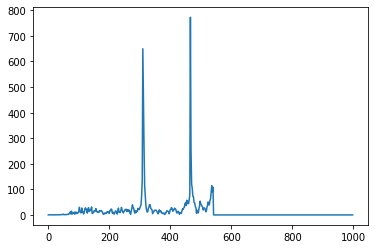
\includegraphics[scale=1]{fig/lab01/lab01_21_0.png}
		\caption{Спект с фильтром нижних частот}
	\end{center}
\end{figure}

Добавим фильтр верхних частот, и ослабим на половину компоненты до 500 Гц.

\begin{lstlisting}[language=Python]
spectrum2.high_pass(500,0.5)
spectrum2.plot(high=1000)
\end{lstlisting}

\begin{figure}[H]
	\begin{center}
		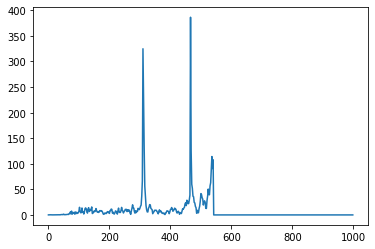
\includegraphics[scale=1]{fig/lab01/lab01_23_0.png}
		\caption{Спект с фильтром верхних частот}
	\end{center}
\end{figure}

Уберём частоты между Ре и Ля.

\begin{lstlisting}[language=Python]
spectrum2.band_stop(320,450)
spectrum2.plot(high=1000)
\end{lstlisting}



\begin{figure}[H]
	\begin{center}
		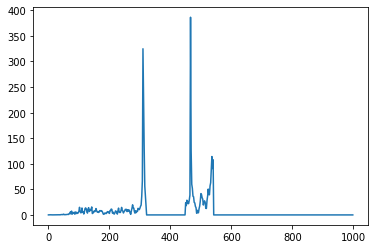
\includegraphics[scale=1]{fig/lab01/lab01_25_0.png}
		\caption{Получившийся спектр}
	\end{center}
\end{figure}

Звучание заметно изменилось из-за изменения доиминирующей частоты (её ампилитуда была уменьшена в 2 раза), но напоминает изначальный отрезок.

\begin{lstlisting}[language=Python]
wave = read_wave('164718__bradovic__piano.wav')
wave = wave.segment(18.3,0.5)
spectrum2 = wave.make_spectrum()
spectrum2.high_pass(500)
spectrum2.plot(high=1000)
\end{lstlisting}

\begin{figure}[H]
	\begin{center}
		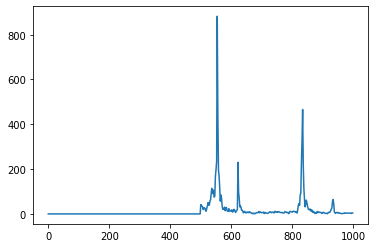
\includegraphics[scale=1]{fig/lab01/lab01_28_0.png}
		\caption{Отфилтрованные нижние компоненты}
	\end{center}
\end{figure}

Отфильтровав нижние частоты звук стал более высоким.

\subsection{Упражнение 2}

Создайте сложный сигнал из объектов SinSignal и CosSignal, суммируя их. Обработайте сигнал для получения wave и прослушайте его. Вычислите Spectrum и распечатайте. Что произойдёт при добавлении частотных компонент, не кратных основным?


Берём два сигнала с частотой одной октавы.
\begin{lstlisting}[language=Python]
from thinkdsp import SinSignal, CosSignal
# https://nch-nch.ru/apps/frequency/
cos_sig1 = CosSignal(freq=784.00,amp=1,offset=0)
sin_sig2 = CosSignal(freq=392.00,amp=0.5,offset=0)
mix = cos_sig1 + sin_sig2
wave = mix.make_wave(duration=1)
wave.make_audio()
\end{lstlisting}

\begin{figure}[H]
	\begin{center}
		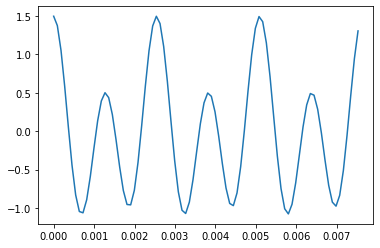
\includegraphics[scale=1]{fig/lab01/lab01_34_0.png}
		\caption{Суммированные сигналы}
	\end{center}
\end{figure}

\begin{lstlisting}[language=Python]
spectrum = wave.make_spectrum()
spectrum.plot(high = 1000)
\end{lstlisting}

\begin{figure}[H]
	\begin{center}
		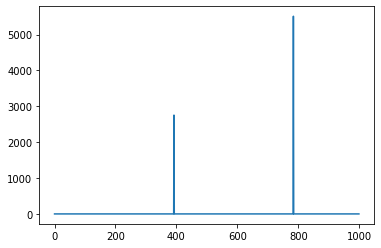
\includegraphics[scale=1]{fig/lab01/lab01_35_0.png}
		\caption{Спектр сигнала}
	\end{center}
\end{figure}

Добавим частоту из другой октавы. Должно получится ужасно для ушей.

\begin{lstlisting}[language=Python]
cos_signal3 = CosSignal(freq = 500, amp=0.25,offset = 0)
mix = mix + cos_signal3
wave = mix.make_wave(duration=1)
wave.make_audio()
\end{lstlisting}

На графике за 7мс не видно цикла.
\begin{figure}[H]
	\begin{center}
		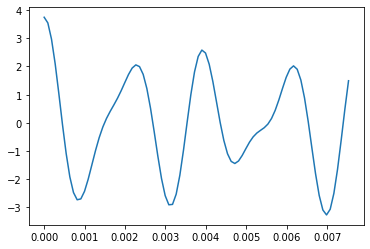
\includegraphics[scale=1]{fig/lab01/lab01_39_0.png}
		\caption{Получившийся сигнал}
	\end{center}
\end{figure}

Действительно, звук очень неприятный.


\subsection{Упражнение 3}

Напишите функцию strech, берущую wave и коэффицент изменения. Она должна ускорять или замедлять сигнал изменением ts и framerate.

\noindent ts - отвечает за моменты выборки сигнала framerate - число выборок в единицу времени.

\noindent Если умножим ts на k, то интервалы между моментами увеличатся в k раз.

\noindent Если framerate поделим на k, то будет меньшее число подвыборок.

\begin{lstlisting}[language=Python]
def stretch(wave, k):
  wave.ts *= k
  wave.framerate /= k
  return wave 
\end{lstlisting}


\subsection{Вывод}
В ходе данной работы было выполнено знакомство с основыми понятиями при работе со звуками и сигналами. При помощи библиотеки thinkDSP можно делать обширный круг взаимодействий с сигналами, как для их создания, так и для их обработки.